% Created 2016-01-08 Fri 17:05
\documentclass[bigger]{beamer}
\usepackage[utf8]{inputenc}
\usepackage[T1]{fontenc}
\usepackage{fixltx2e}
\usepackage{graphicx}
\usepackage{grffile}
\usepackage{longtable}
\usepackage{wrapfig}
\usepackage{rotating}
\usepackage[normalem]{ulem}
\usepackage{amsmath}
\usepackage{textcomp}
\usepackage{amssymb}
\usepackage{capt-of}
\usepackage{hyperref}
\usepackage{minted}
\usepackage{inconsolata}
\usepackage{tikz}
\usepgflibrary{shapes.geometric}
\usetikzlibrary{calc}
\usetikzlibrary{positioning}
\usetikzlibrary{plotmarks}
\usepackage{pgfplots}
\institute{Departments of Mathematics and Computing, Imperial College London}
\AtBeginSection[]{\begin{frame}\tableofcontents[currentsection]\end{frame}}
\usetheme{IC}
\author{\textbf{Lawrence Mitchell}, Gheorghe-Teodor Bercea, David Ham, Paul Kelly, Nicolas Loriant, Fabio Luporini, Florian Rathgeber}
\date{21 February 2014}
\title{Firedrake: a multilevel domain specific language approach to unstructured mesh stencil computations}
\hypersetup{
 pdfauthor={\textbf{Lawrence Mitchell}, Gheorghe-Teodor Bercea, David Ham, Paul Kelly, Nicolas Loriant, Fabio Luporini, Florian Rathgeber},
 pdftitle={Firedrake: a multilevel domain specific language approach to unstructured mesh stencil computations},
 pdfkeywords={},
 pdfsubject={},
 pdfcreator={Emacs 24.5.1 (Org mode 8.3.2)}, 
 pdflang={English}}
\begin{document}

\maketitle

\section{Introduction}
\label{sec:orgheadline3}

\begin{frame}[label={sec:orgheadline1}]{What are we interested in?}
\begin{itemize}
\item (Predominantly) finite element simulations
\begin{itemize}
\item primary application areas in geophysical fluids (ocean and
atmosphere)
\item simulations on unstructured and semi-structured meshes
\end{itemize}
\item Providing high-level interfaces for users, with performance
\end{itemize}
\pause
\begin{itemize}
\item the moon, on a stick
\end{itemize}
\end{frame}

\begin{frame}[label={sec:orgheadline2}]{What are the elementary operations?}
\begin{itemize}
\item \emph{Numerics} tell us the elementary operation we apply everywhere in
the mesh (a "kernel")
\item \emph{Mesh topology} gives us the "stencil" pattern
\item Our job: efficiently apply the kernel over the whole mesh
\end{itemize}

\begin{center}
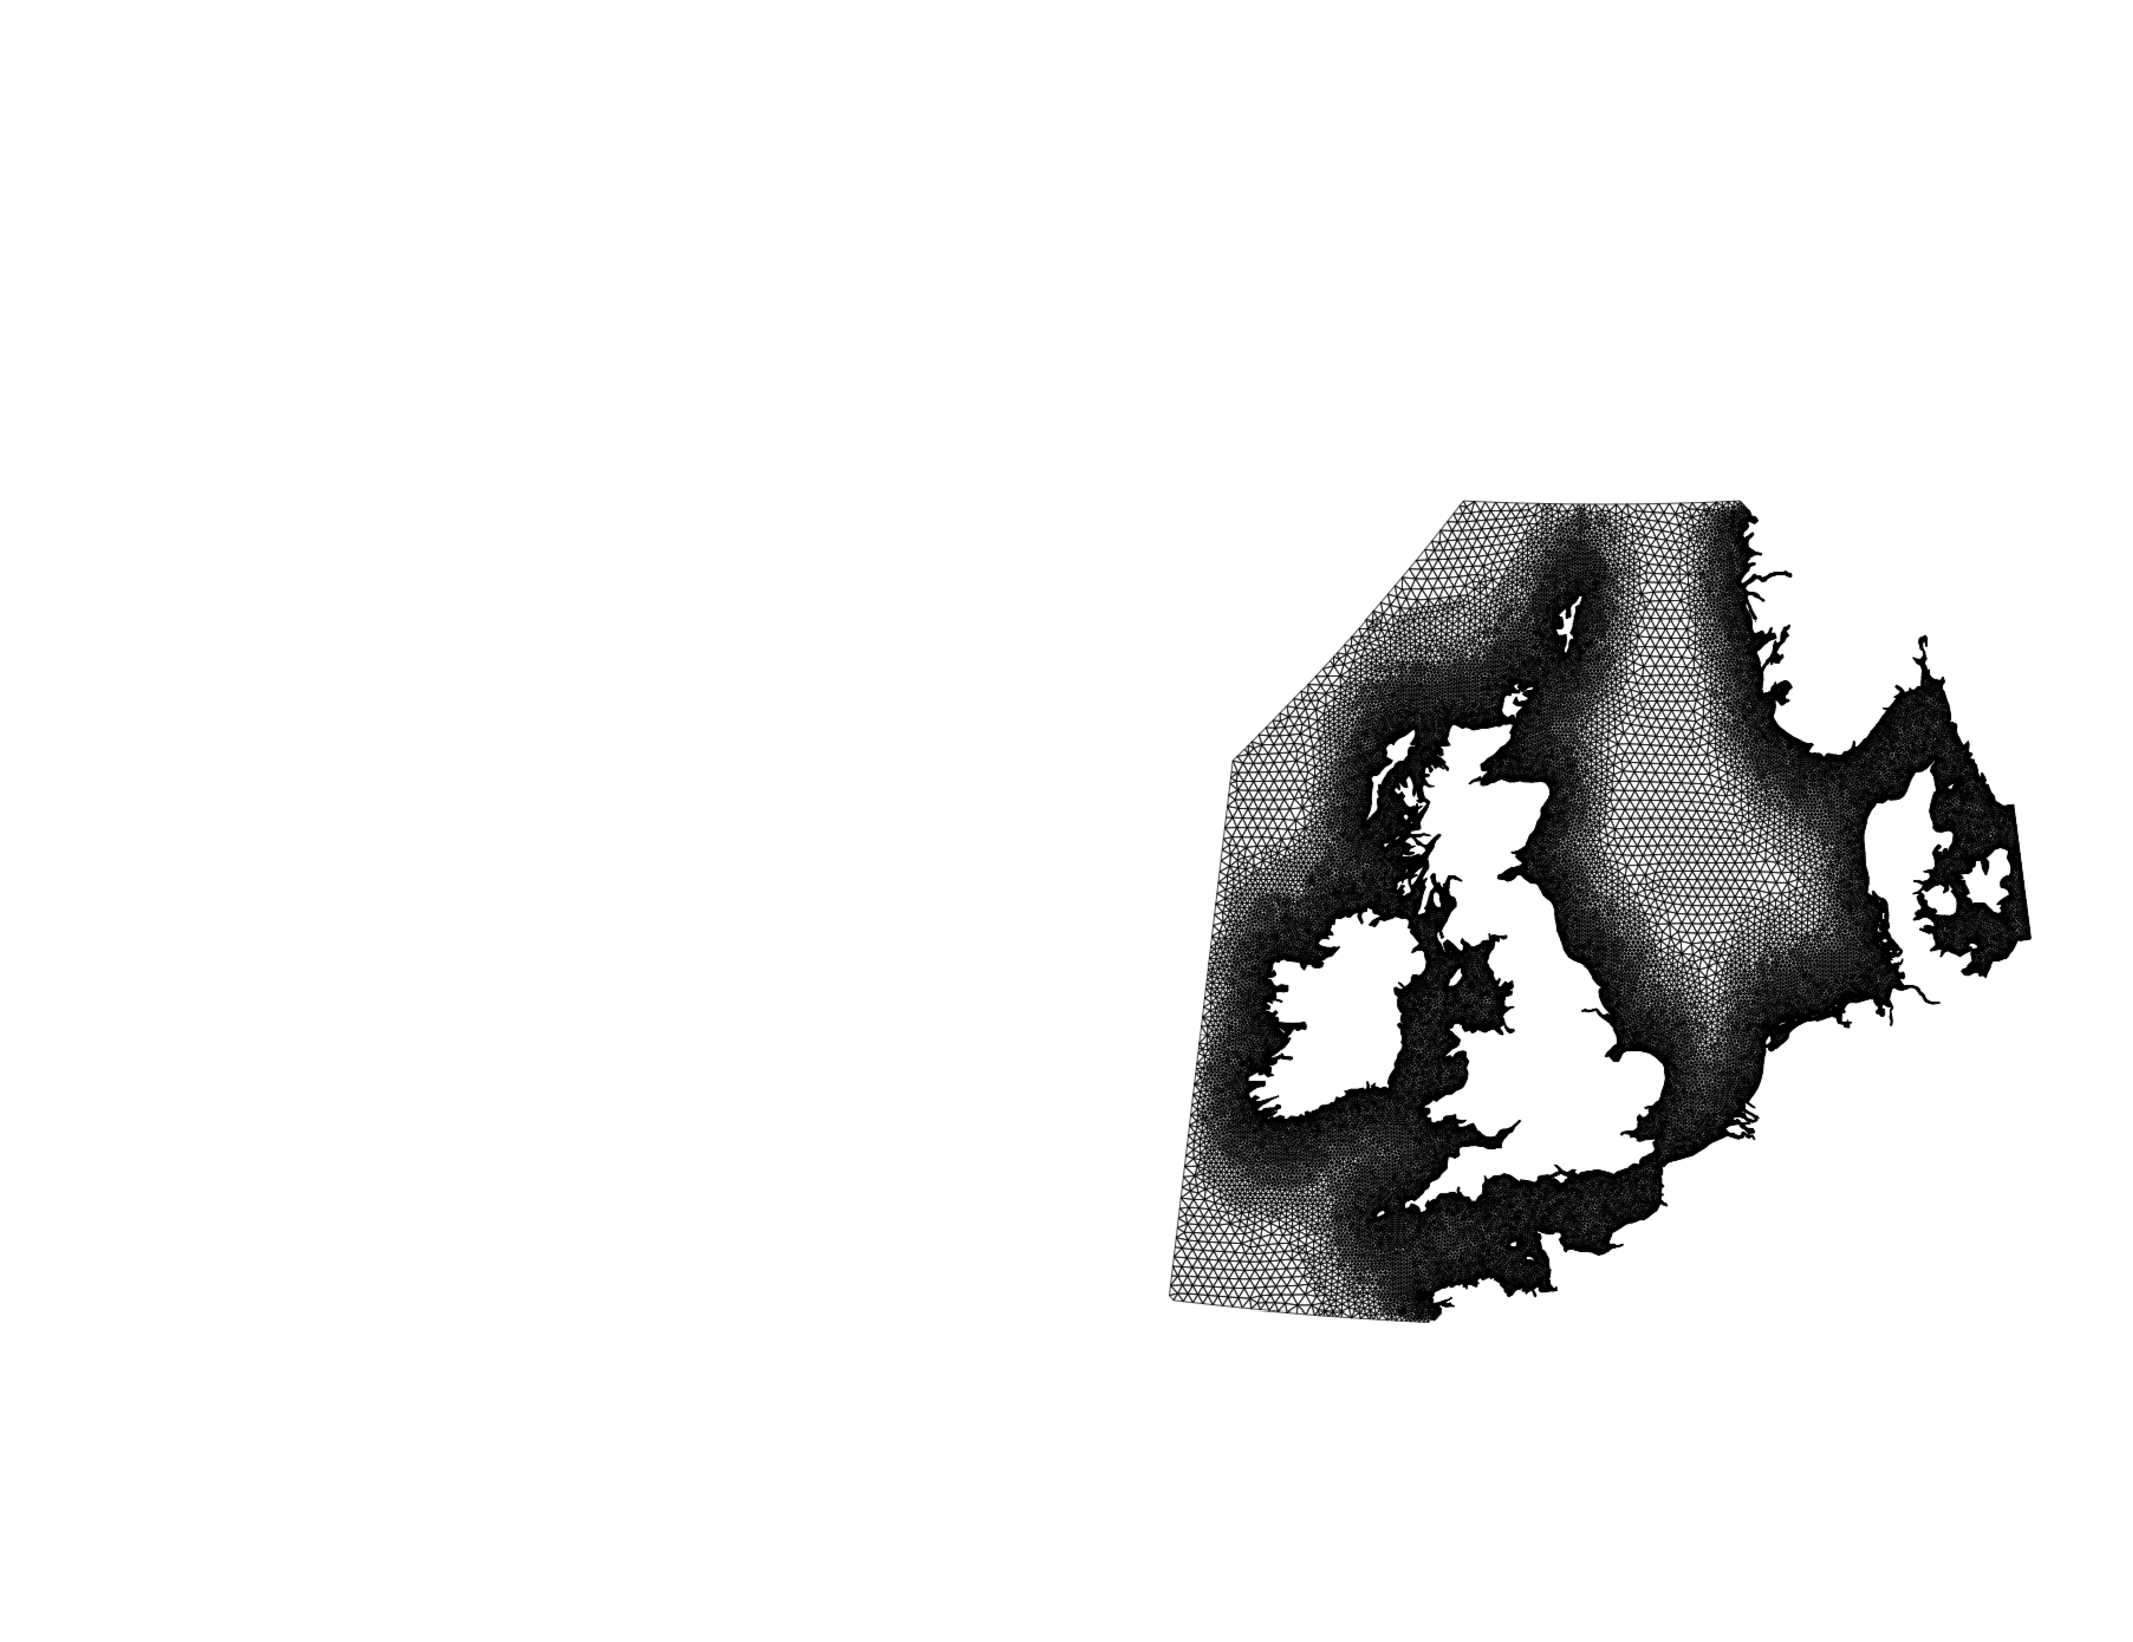
\includegraphics[height=0.75\textheight]{02-22-SIAM-PP-extruded-meshes.figures/uk-mesh}
\end{center}
\end{frame}
\section{Maintaining abstractions}
\label{sec:orgheadline10}

\begin{frame}[label={sec:orgheadline4}]{Express what, not how}
\begin{itemize}
\item User code should make as few decisions about implementation as
possible
\item FE discretisations expressed symbolically using the \emph{Unified Form Language}
\begin{itemize}
\item developed in the FEniCS project (\url{http://www.fenicsproject.org})
\item symbolic representation compiled to a C kernel
\end{itemize}
\item Data to feed to kernel (and interface to solvers) provided by
Firedrake (\url{http://www.firedrakeproject.org})
\item Execution of kernel over entire domain expressed as parallel loop
with access descriptors
\begin{itemize}
\item uses PyOP2 unstructured mesh library (\url{http://github.com/OP2/PyOP2})
\end{itemize}
\end{itemize}
\end{frame}

\begin{frame}[plain,label={sec:orgheadline5}]{Firedrake}
\begin{center}
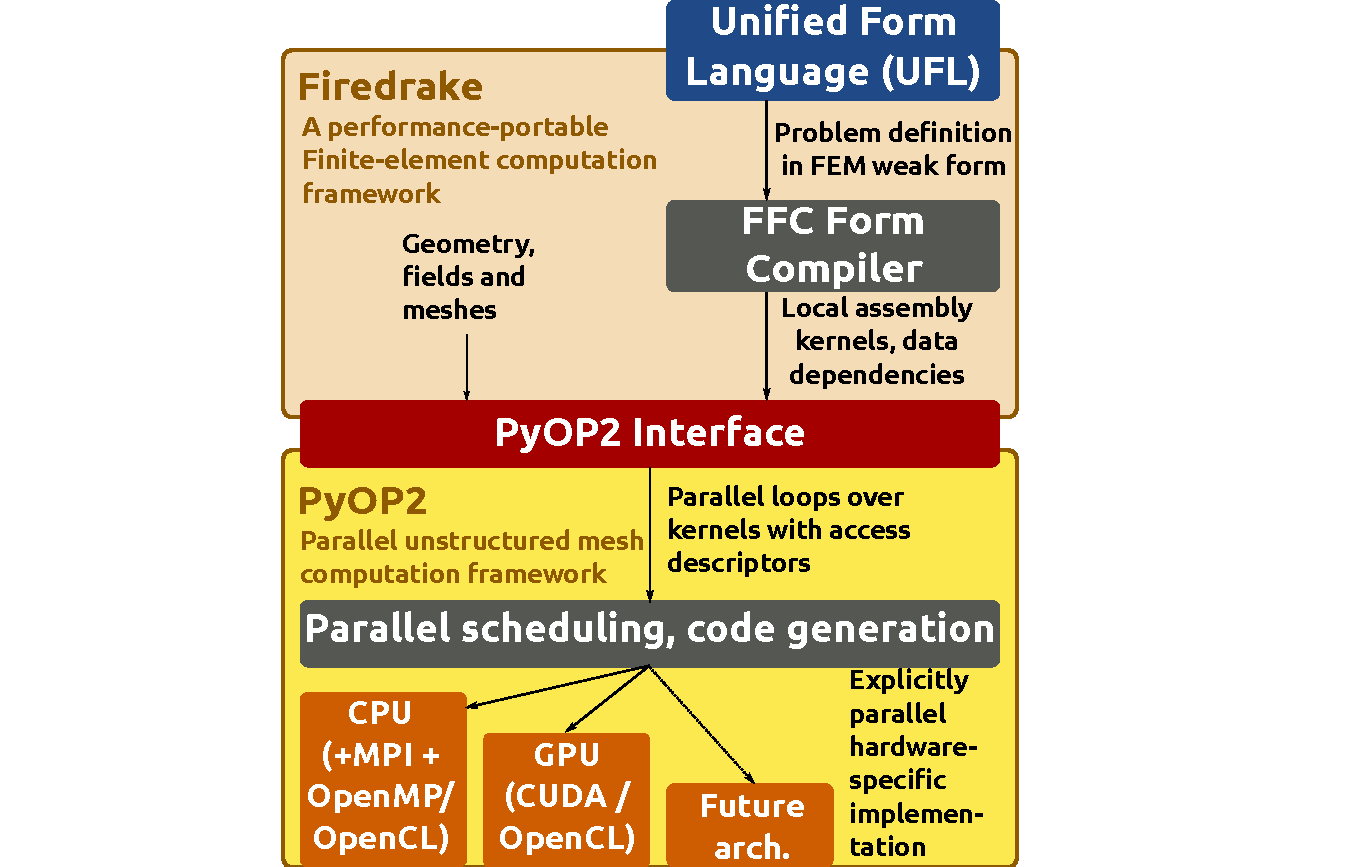
\includegraphics[height=1\textheight]{02-22-SIAM-PP-extruded-meshes.figures/firedrake_toolchain}
\end{center}
\end{frame}

\begin{frame}[fragile,label={sec:orgheadline6}]{An example}
 \begin{minted}[frame=none,xleftmargin=1em,xrightmargin=1em,fontsize=\scriptsize,mathescape]{python}
from firedrake import *
m = UnitSquareMesh(32, 32)
V = FunctionSpace(m, 'Lagrange', 2)
u = Function(V)
v = TestFunction(V)
# $F(u;v)=\int\nabla{}u\cdot\nabla{}v+uv\mathrm{d}x$
F = inner(grad(u), grad(v))*dx + u*v*dx
solve(F == 0, u)
\end{minted}
\begin{itemize}
\item Kernels produced for residual and jacobian evaluation
\begin{itemize}
\item jacobian computed by symbolic differentiation of
residual form
\end{itemize}
\item Kernels executed over mesh using PyOP2
\begin{itemize}
\item \url{http://github.com/OP2/PyOP2}
\end{itemize}
\end{itemize}
\end{frame}

\begin{frame}[fragile,label={sec:orgheadline7}]{PyOP2 data model}
 \begin{itemize}
\item Data types
\begin{description}
\item[{\emph{Set}}] e.g. cells, degrees of freedom (dofs)
\item[{\emph{Dat}}] data defined on a \texttt{Set} (one entry per set element)
\item[{\emph{Map}}] a mapping between two sets (e.g. cells to dofs), a "stencil"
\item[{\emph{Global}}] global data (one entry)
\item[{\emph{Kernel}}] a piece of code to execute over the mesh (in C)
\end{description}
\item access descriptors
\begin{itemize}
\item READ, RW, WRITE, INC, \ldots{}
\end{itemize}
\item iteration construct
\begin{description}
\item[{\emph{\texttt{par\_loop}}}] execute a Kernel over every element in a \texttt{Set}
\end{description}
\end{itemize}
\end{frame}

\begin{frame}[fragile,label={sec:orgheadline8}]{Example}
 \begin{minted}[frame=none,xleftmargin=1em,xrightmargin=1em,fontsize=\scriptsize,mathescape]{python}
elements = Set(...)
nodes = Set(...)
elem_node = Map(elements, nodes, 3, ...) # 3 nodes per element
node_data = Dat(nodes, ...)
element_data = Dat(elements, ...)
count = Global(...)                 # no set (global value)
par_loop(kernel, elements,
         element_data(READ),        # direct read
         node_data(INC, elem_node), # indirect increment
         count(INC))                # global increment
\end{minted}
\begin{itemize}
\item executes \emph{kernel} for each ele in \emph{elements}
\item runtime knows it has to care about data dependencies for
\begin{itemize}
\item increments into \texttt{node\_data}
\item increment into \texttt{count}
\end{itemize}
\end{itemize}
\end{frame}

\begin{frame}[label={sec:orgheadline9}]{Synthesis, not analysis}
\begin{itemize}
\item Low level code is generated at runtime for parallel loops
\item Access descriptors on parallel loops mean:
\begin{itemize}
\item code generation requires synthesis, not analysis
\item determination of when halo exchanges need to occur is automatic
\item colouring for shared memory parallelisation can be computed
automatically
\end{itemize}
\end{itemize}

\pause
\begin{center}
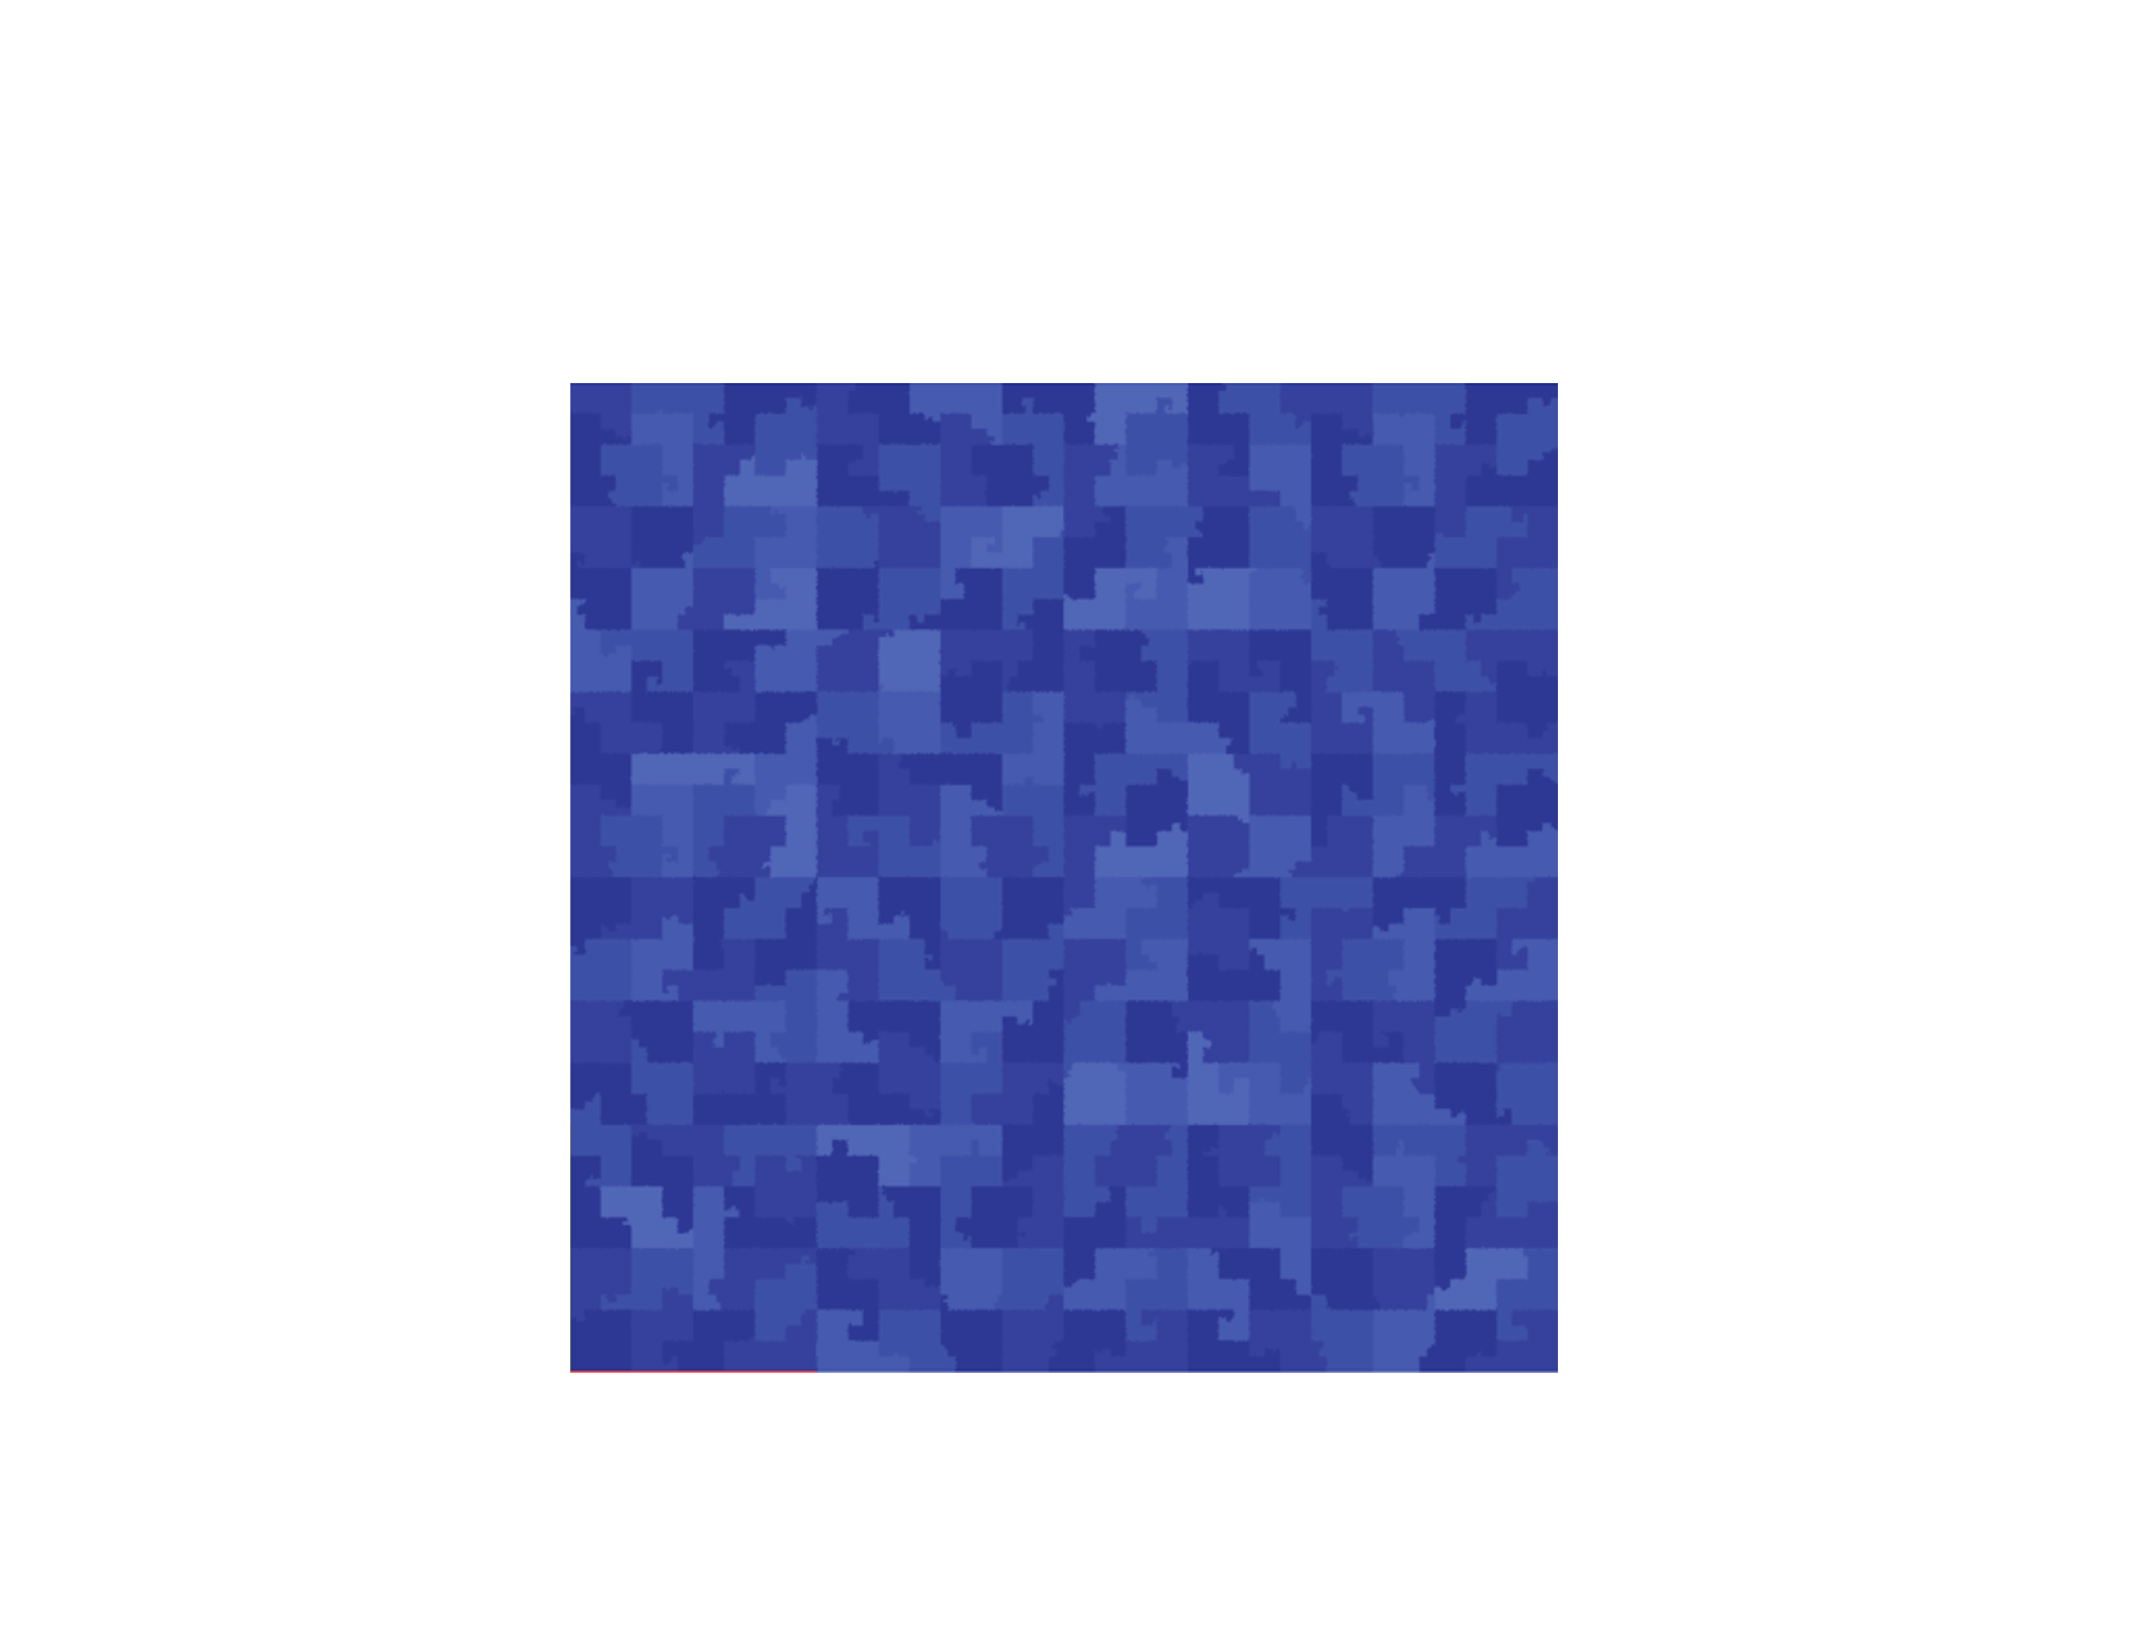
\includegraphics[height=0.6\textheight]{02-22-SIAM-PP-extruded-meshes.figures/mesh-colouring}
\end{center}
\end{frame}

\section{Exploiting structure}
\label{sec:orgheadline14}

\begin{frame}[label={sec:orgheadline11}]{Semi-structured meshes}
\begin{itemize}
\item Many application areas have a "short" direction
\begin{itemize}
\item ocean and atmosphere
\item thin shells
\end{itemize}
\item Numerics dictate we should do something different in short
direction
\item Use semi-structured meshes
\begin{itemize}
\item unstructured in "long" directions, structured in short
\item can we exploit this structure?
\end{itemize}
\end{itemize}
\end{frame}

\begin{frame}[label={sec:orgheadline12}]{A picture of triangles}
\begin{center}
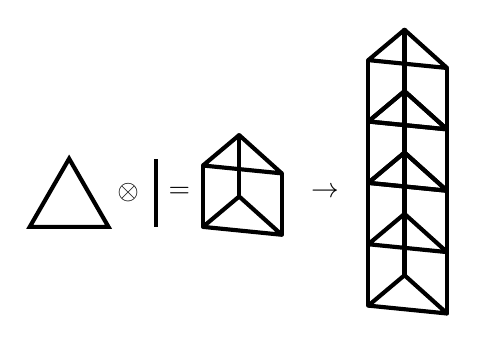
\begin{tikzpicture}[scale=1]
\draw[line width=1.5pt] (0,0) -- (1,0) -- (60:1) -- cycle;
\node at (1.25,0 |- 60:0.5) {$\otimes$};
\draw[line width=1.5pt] (1.6,0) -- (1.6,0 |- 60:1);
\node at (1.9,0 |- 60:0.5) {$=$};

\draw[line width=1.5pt, line join=bevel] (2.2,0) -- +(1, -0.1) -- +(40:0.6) -- cycle;

\draw[line width=1.5pt, line cap=round] (2.2, 0) -- +(0,0 |- 60:0.9);
\draw[line width=1.5pt, line cap=round] (2.2, 0) ++(1, -0.1) -- +(0,0 |- 60:0.9);
\draw[line width=1.5pt, line cap=round] (2.2, 0) ++(40:0.6) -- +(0,0 |- 60:0.9);
\draw[line width=1.5pt, line join=bevel] (2.2,0) ++(0,0 |- 60:0.9) --
+(1, -0.1) -- +(40:0.6) -- cycle;

\node at (3.75, 0 |- 60:0.5) {$\rightarrow$};
% ++(0,0 |- 60:1) -- +(1, -0.25) -- +(40:0.7) -- (2, 0 |- 60:1);

\draw[line width=1.5pt, line join=bevel] (4.3, -1) -- +(1, -0.1) -- +(40:0.6) -- cycle;
\draw[line width=1.5pt, line cap=round] (4.3, -1) -- +(0,0 |- 60:0.9);
\draw[line width=1.5pt, line cap=round] (4.3, -1) ++(1, -0.1) -- +(0,0 |- 60:0.9);
\draw[line width=1.5pt, line cap=round] (4.3, -1) ++(40:0.6) -- +(0,0 |- 60:0.9);
\draw[line width=1.5pt, line join=bevel] (4.3, -1) ++(0,0 |- 60:0.9) -- +(1, -0.1) -- +(40:0.6) -- cycle;

\draw[line width=1.5pt, line cap=round] (4.3, -1) ++(0,0 |- 60:0.9) -- +(0,0 |- 60:0.9);
\draw[line width=1.5pt, line cap=round] (4.3, -1) ++(0,0 |- 60:0.9) ++(1, -0.1) -- +(0,0 |- 60:0.9);
\draw[line width=1.5pt, line cap=round] (4.3, -1) ++(0,0 |- 60:0.9) ++(40:0.6) -- +(0,0 |- 60:0.9);
\draw[line width=1.5pt, line join=bevel] (4.3, -1) ++(0,0 |- 60:0.9) ++(0,0 |- 60:0.9) -- +(1, -0.1) -- +(40:0.6) -- cycle;

\draw[line width=1.5pt, line join=bevel] (4.3, -1) ++(0,0 |- 60:1.8) -- +(1, -0.1) -- +(40:0.6) -- cycle;
\draw[line width=1.5pt, line cap=round] (4.3, -1) ++(0,0 |- 60:1.8) -- +(0,0 |- 60:0.9);
\draw[line width=1.5pt, line cap=round] (4.3, -1) ++(0,0 |- 60:1.8) ++(1, -0.1) -- +(0,0 |- 60:0.9);
\draw[line width=1.5pt, line cap=round] (4.3, -1) ++(0,0 |- 60:1.8) ++(40:0.6) -- +(0,0 |- 60:0.9);
\draw[line width=1.5pt, line join=bevel] (4.3, -1) ++(0,0 |- 60:1.8) ++(0,0 |- 60:0.9) -- +(1, -0.1) -- +(40:0.6) -- cycle;

\draw[line width=1.5pt, line join=bevel] (4.3, -1) ++(0,0 |- 60:2.7) -- +(1, -0.1) -- +(40:0.6) -- cycle;
\draw[line width=1.5pt, line cap=round] (4.3, -1) ++(0,0 |- 60:2.7) -- +(0,0 |- 60:0.9);
\draw[line width=1.5pt, line cap=round] (4.3, -1) ++(0,0 |- 60:2.7) ++(1, -0.1) -- +(0,0 |- 60:0.9);
\draw[line width=1.5pt, line cap=round] (4.3, -1) ++(0,0 |- 60:2.7) ++(40:0.6) -- +(0,0 |- 60:0.9);
\draw[line width=1.5pt, line join=bevel] (4.3, -1) ++(0,0 |- 60:2.7) ++(0,0 |- 60:0.9) -- +(1, -0.1) -- +(40:0.6) -- cycle;
\end{tikzpicture}

\end{center}
\end{frame}

\begin{frame}[label={sec:orgheadline13}]{Admits a fast implementation}
\begin{columns}
\begin{column}{0.6\columnwidth}
\begin{itemize}
\item Exploit structure in mesh to amortize indirect lookups
\begin{itemize}
\item arrange for iteration over short direction to be innermost loop
\item pay one indirect lookup per mesh column
\item walk up column directly
\end{itemize}
\end{itemize}
\end{column}

\begin{column}{0.5\columnwidth}
\hfill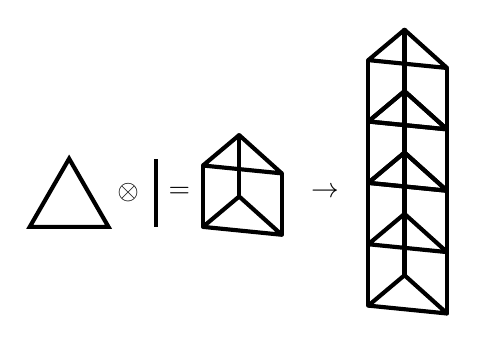
\begin{tikzpicture}[scale=1]
\draw[line width=1.5pt] (0,0) -- (1,0) -- (60:1) -- cycle;
\node at (1.25,0 |- 60:0.5) {$\otimes$};
\draw[line width=1.5pt] (1.6,0) -- (1.6,0 |- 60:1);
\node at (1.9,0 |- 60:0.5) {$=$};

\draw[line width=1.5pt, line join=bevel] (2.2,0) -- +(1, -0.1) -- +(40:0.6) -- cycle;

\draw[line width=1.5pt, line cap=round] (2.2, 0) -- +(0,0 |- 60:0.9);
\draw[line width=1.5pt, line cap=round] (2.2, 0) ++(1, -0.1) -- +(0,0 |- 60:0.9);
\draw[line width=1.5pt, line cap=round] (2.2, 0) ++(40:0.6) -- +(0,0 |- 60:0.9);
\draw[line width=1.5pt, line join=bevel] (2.2,0) ++(0,0 |- 60:0.9) --
+(1, -0.1) -- +(40:0.6) -- cycle;

\node at (3.75, 0 |- 60:0.5) {$\rightarrow$};
% ++(0,0 |- 60:1) -- +(1, -0.25) -- +(40:0.7) -- (2, 0 |- 60:1);

\draw[line width=1.5pt, line join=bevel] (4.3, -1) -- +(1, -0.1) -- +(40:0.6) -- cycle;
\draw[line width=1.5pt, line cap=round] (4.3, -1) -- +(0,0 |- 60:0.9);
\draw[line width=1.5pt, line cap=round] (4.3, -1) ++(1, -0.1) -- +(0,0 |- 60:0.9);
\draw[line width=1.5pt, line cap=round] (4.3, -1) ++(40:0.6) -- +(0,0 |- 60:0.9);
\draw[line width=1.5pt, line join=bevel] (4.3, -1) ++(0,0 |- 60:0.9) -- +(1, -0.1) -- +(40:0.6) -- cycle;

\draw[line width=1.5pt, line cap=round] (4.3, -1) ++(0,0 |- 60:0.9) -- +(0,0 |- 60:0.9);
\draw[line width=1.5pt, line cap=round] (4.3, -1) ++(0,0 |- 60:0.9) ++(1, -0.1) -- +(0,0 |- 60:0.9);
\draw[line width=1.5pt, line cap=round] (4.3, -1) ++(0,0 |- 60:0.9) ++(40:0.6) -- +(0,0 |- 60:0.9);
\draw[line width=1.5pt, line join=bevel] (4.3, -1) ++(0,0 |- 60:0.9) ++(0,0 |- 60:0.9) -- +(1, -0.1) -- +(40:0.6) -- cycle;

\draw[line width=1.5pt, line join=bevel] (4.3, -1) ++(0,0 |- 60:1.8) -- +(1, -0.1) -- +(40:0.6) -- cycle;
\draw[line width=1.5pt, line cap=round] (4.3, -1) ++(0,0 |- 60:1.8) -- +(0,0 |- 60:0.9);
\draw[line width=1.5pt, line cap=round] (4.3, -1) ++(0,0 |- 60:1.8) ++(1, -0.1) -- +(0,0 |- 60:0.9);
\draw[line width=1.5pt, line cap=round] (4.3, -1) ++(0,0 |- 60:1.8) ++(40:0.6) -- +(0,0 |- 60:0.9);
\draw[line width=1.5pt, line join=bevel] (4.3, -1) ++(0,0 |- 60:1.8) ++(0,0 |- 60:0.9) -- +(1, -0.1) -- +(40:0.6) -- cycle;

\draw[line width=1.5pt, line join=bevel] (4.3, -1) ++(0,0 |- 60:2.7) -- +(1, -0.1) -- +(40:0.6) -- cycle;
\draw[line width=1.5pt, line cap=round] (4.3, -1) ++(0,0 |- 60:2.7) -- +(0,0 |- 60:0.9);
\draw[line width=1.5pt, line cap=round] (4.3, -1) ++(0,0 |- 60:2.7) ++(1, -0.1) -- +(0,0 |- 60:0.9);
\draw[line width=1.5pt, line cap=round] (4.3, -1) ++(0,0 |- 60:2.7) ++(40:0.6) -- +(0,0 |- 60:0.9);
\draw[line width=1.5pt, line join=bevel] (4.3, -1) ++(0,0 |- 60:2.7) ++(0,0 |- 60:0.9) -- +(1, -0.1) -- +(40:0.6) -- cycle;
\end{tikzpicture}

\end{column}
\end{columns}
\end{frame}

\section{Benchmarking}
\label{sec:orgheadline23}
\begin{frame}[fragile,label={sec:orgheadline15}]{A bandwidth bound test}
 \begin{itemize}
\item Walk over mesh, read from vertices and cells, sum into global
\end{itemize}
\begin{minted}[frame=none,xleftmargin=1em,xrightmargin=1em,fontsize=\scriptsize,mathescape]{c}
void kernel(double *a, double *x[], double *y[]) {
    const double area = fabs(x[0][0]*(x[2][1]-x[4][1])
                             + x[2][0]*(x[4][1]-x[0][1])
                             + x[4][0]*(x[0][1]-x[2][1]));
    *a += area * 0.5 * y[0][0];
}
\end{minted}
\begin{itemize}
\item Can we sustain an appreciable fraction of memory bandwidth?
\end{itemize}
\end{frame}

\begin{frame}[label={sec:orgheadline16}]{Measuring throughput}
\begin{itemize}
\item "Effective" data volume
\begin{itemize}
\item assume every piece of data is touched exactly once (in perfect
order)
\item don't count data movement for indirection maps
\end{itemize}
\item "Valuable" bandwidth
\begin{itemize}
\item effective data volume per second
\end{itemize}
\item Actual memory bandwidth will be higher (reading indirection maps)
\begin{itemize}
\item but this is not "useful"
\end{itemize}
\end{itemize}
\end{frame}

\begin{frame}[label={sec:orgheadline17}]{Benchmark setup}
\begin{itemize}
\item 2D unstructured mesh: 806110 cells, 403811 vertices.
\begin{itemize}
\item 2D coordinate field located at vertices (implicit 3rd coordinate)
\item scalar field stored at cell centres
\end{itemize}
\item Run with increasing number of extruded cell layers (n\(_{\text{layer}}\))
\begin{itemize}
\item data volume
(806110 * n\(_{\text{layer}}\)) + 403811 * 2 (n\(_{\text{layer}}\) + 1) doubles
\item 1 layer: 18.4MB
\item 200 layers: 2468MB
\end{itemize}
\item Execute kernel over mesh 100 times
\end{itemize}
\end{frame}

\begin{frame}[label={sec:orgheadline18}]{Single node}
\begin{itemize}
\item Intel Sandybridge 4 cores (2 way hyperthreading)
\begin{itemize}
\item 32kB L1 cache (per core)
\item 256 kB L2 cache (per core)
\item 8 MB L3 cache (shared)
\end{itemize}
\item Measured STREAM bandwidth (8 threads)
\begin{itemize}
\item 11341 MB/s
\end{itemize}
\end{itemize}
\end{frame}

\begin{frame}[label={sec:orgheadline19}]{Effect of good base numbering}
\begin{itemize}
\item Being completely unstructured hurts a lot
\item Compare default (mesh generator) numbering with renumbered mesh
using 2D space filling curve
\end{itemize}
\begin{center}
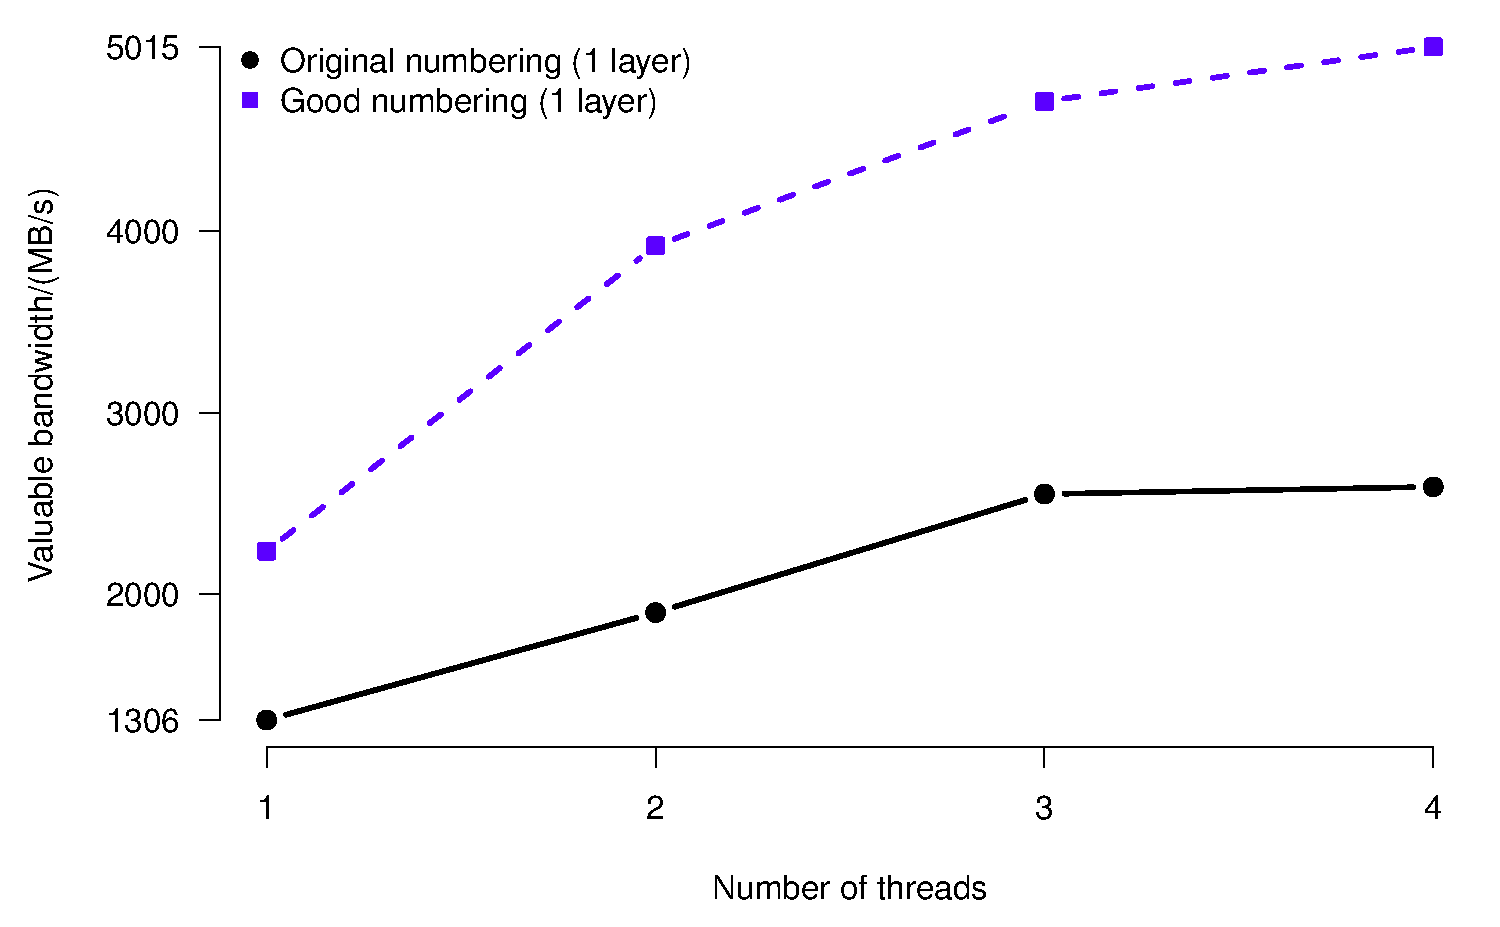
\includegraphics[height=0.8\textheight]{02-22-SIAM-PP-extruded-meshes.figures/bad-numbering}
\end{center}
\end{frame}

\begin{frame}[label={sec:orgheadline20}]{Adding layers amortizes indirection cost}
\begin{itemize}
\item L3 cache bandwidth
\begin{itemize}
\item low layer numbers hit the L3 more often (indirection lookups)
\end{itemize}
\end{itemize}
\begin{center}
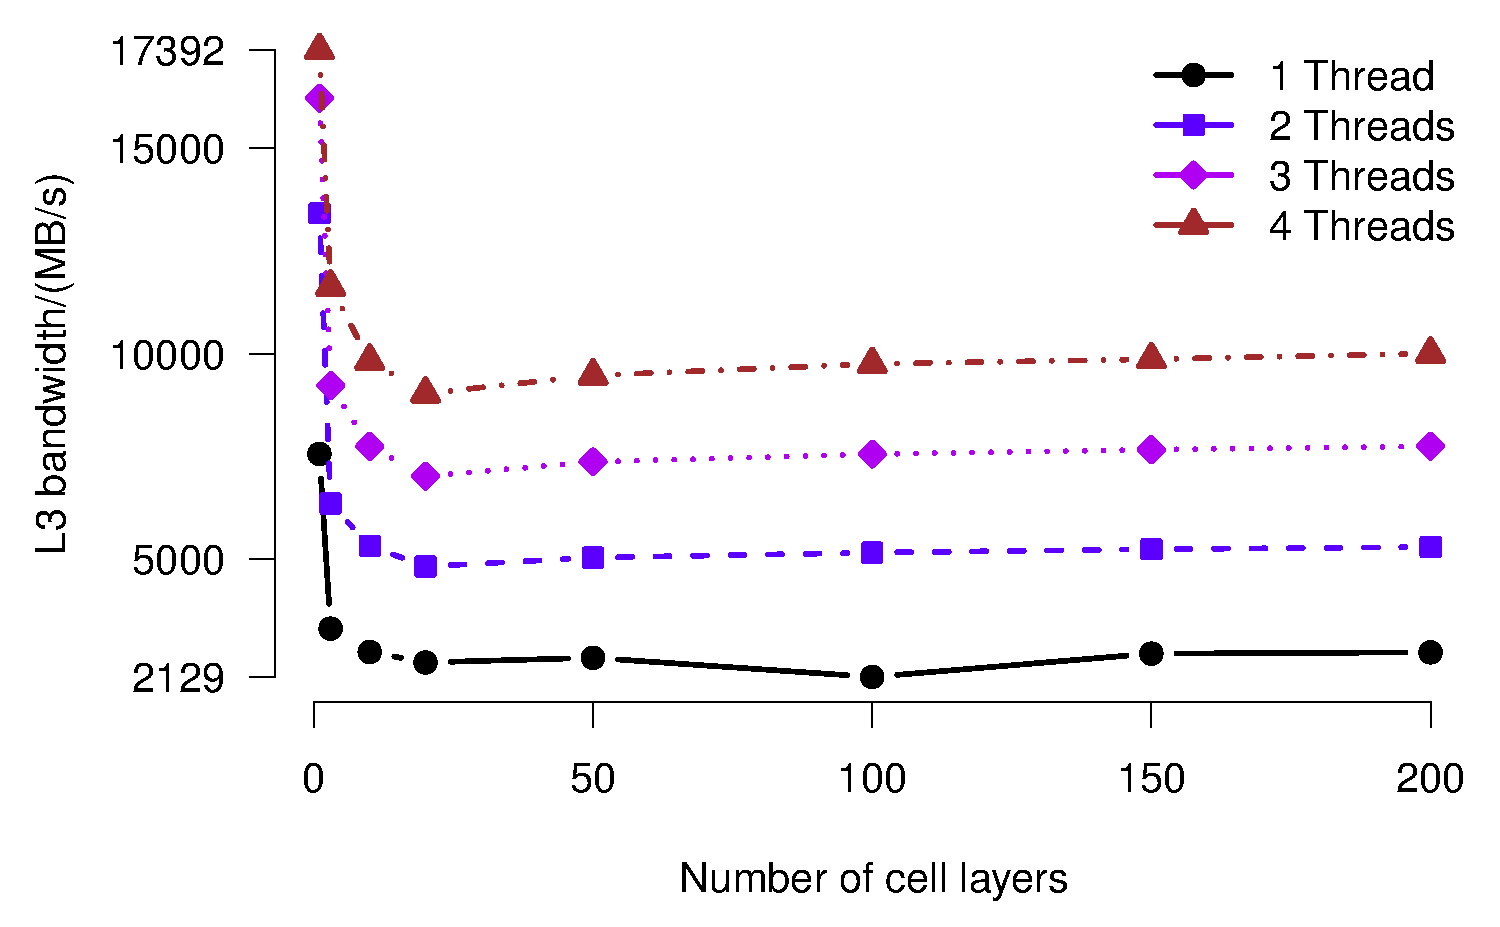
\includegraphics[height=0.6\textheight]{02-22-SIAM-PP-extruded-meshes.figures/L3-bandwidth}
\end{center}
\begin{itemize}
\item What about actual throughput though?
\end{itemize}
\end{frame}

\begin{frame}[label={sec:orgheadline21}]{Valuable bandwidth}
\begin{itemize}
\item Above \textasciitilde{}20 layers, indirection cost "hidden"
\end{itemize}
\begin{center}
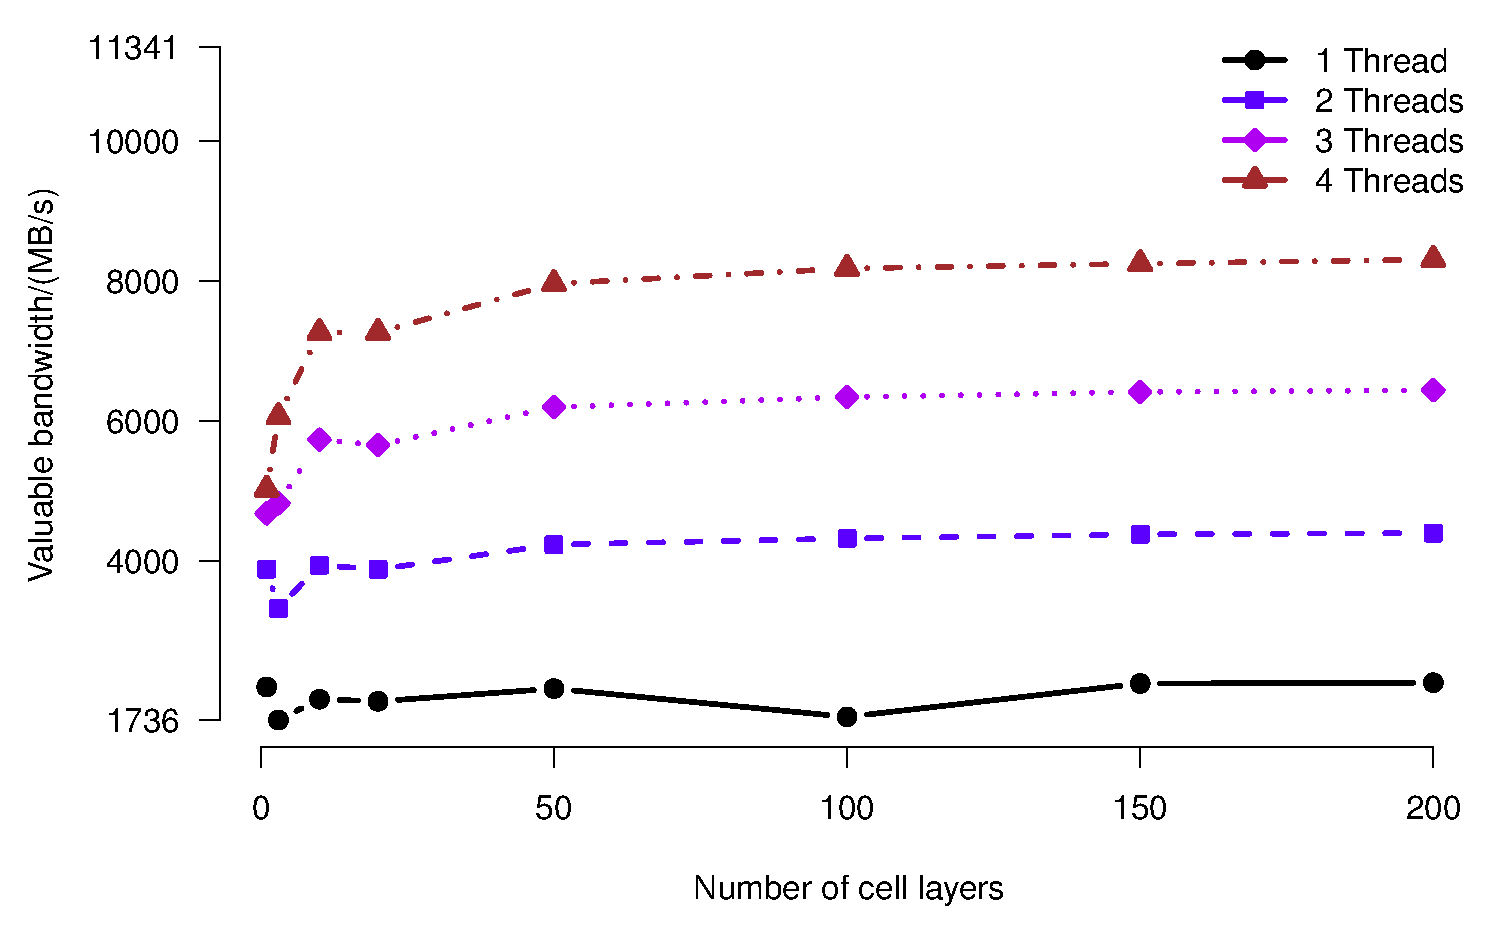
\includegraphics[height=0.8\textheight]{02-22-SIAM-PP-extruded-meshes.figures/valuable-bandwidth-by-layer}
\end{center}
\end{frame}
\begin{frame}[label={sec:orgheadline22}]{More threads}
\begin{itemize}
\item Hyperthreading gives some further gains (82\% STREAM bandwidth)
\end{itemize}
\begin{center}
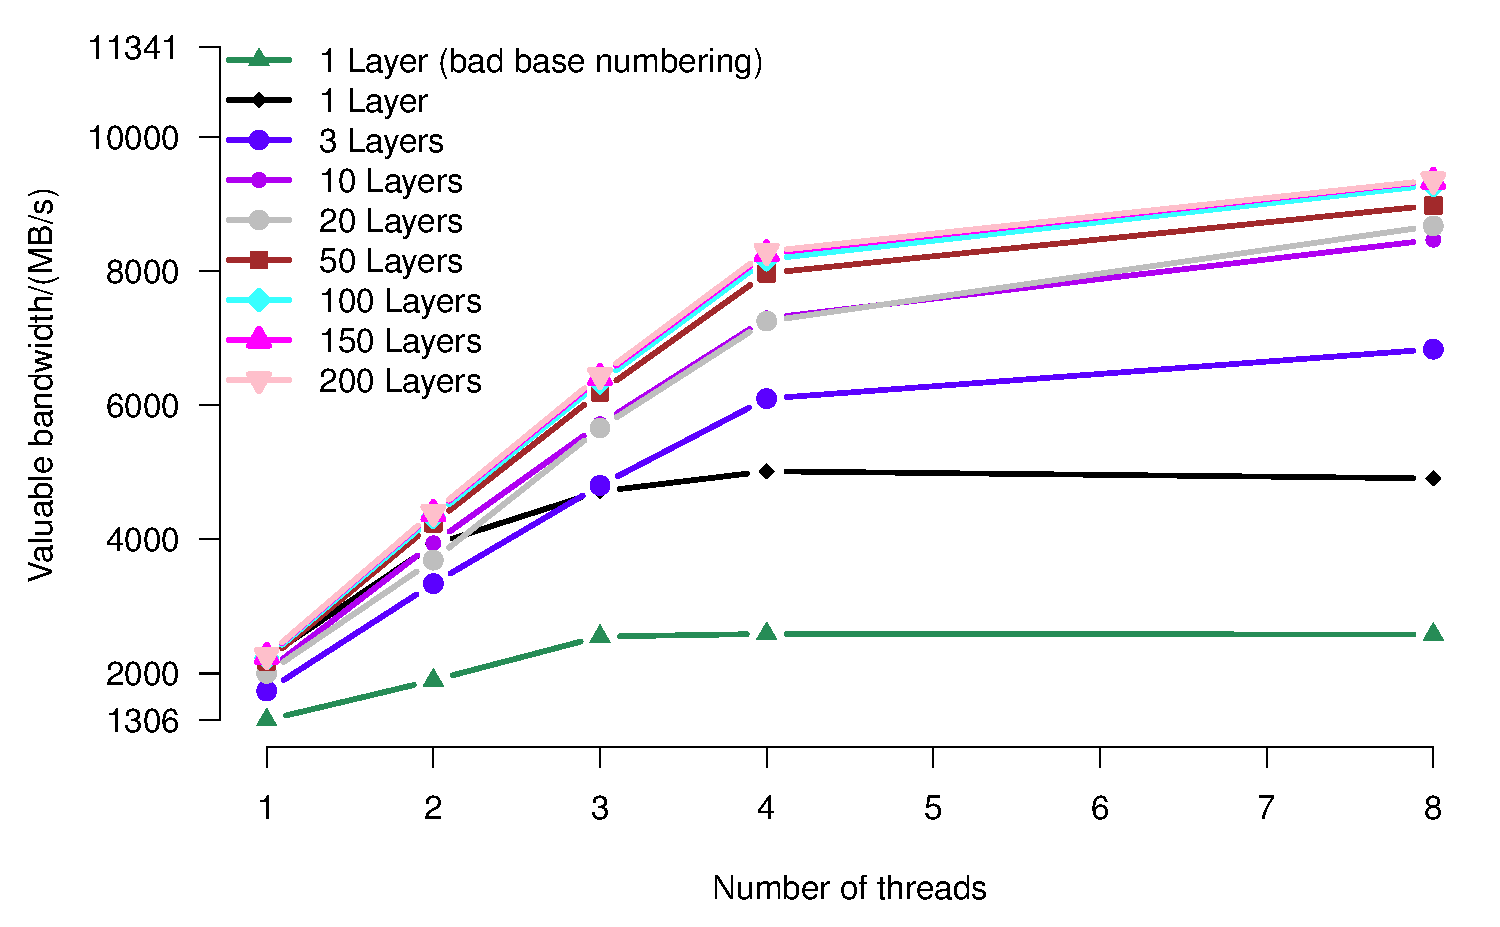
\includegraphics[height=0.8\textheight]{02-22-SIAM-PP-extruded-meshes.figures/valuable-bandwidth-by-thread}
\end{center}
\end{frame}

\section{Conclusions}
\label{sec:orgheadline27}

\begin{frame}[label={sec:orgheadline24}]{Possible to be unstructured and fast}
\begin{itemize}
\item A good numbering gets you a reasonable way there
\item If there is structure in your problem, use it!
\item High level abstractions need not kill performance
\end{itemize}
\end{frame}

\begin{frame}[label={sec:orgheadline25}]{Work with us}
\begin{itemize}
\item All code is open source, and online:
\begin{description}
\item[{Firedrake}] \url{http://www.firedrakeproject.org} and
\url{http://github.com/firedrakeproject/firedrake}
\item[{PyOP2}] \url{http://github.com/OP2/PyOP2} (documentation at
\url{http://op2.github.io/PyOP2})
\end{description}
\item Postdoc positions in this area are available
\begin{itemize}
\item contact: me (lawrence.mitchell@imperial.ac.uk) or David Ham
(david.ham@imperial.ac.uk)
\end{itemize}
\end{itemize}
\end{frame}

\begin{frame}[label={sec:orgheadline26}]{Thanks}
\begin{itemize}
\item Institutions
\begin{itemize}
\item Imperial College London
\item Grantham Institute for climate change
\end{itemize}
\item Funding
\begin{itemize}
\item NERC (NE/K008951/1, NE/K006789/1, NE/G523512/1)
\item EPSRC (EP/L000407/1, EP/K008730/1, EP/I00677X/1)
\end{itemize}
\end{itemize}
\end{frame}
\end{document}
